\section{Introduction}

Mobile apps are utilized for virtually all aspects of daily life in the modern world. So after we noticed that there is no application that allows the efficient planning of campaigns like the "Sternsinger-Aktion" we asked ourselves why, and furthermore, how hard it is to create an App with intuitive usability with the main purpose of simplifying the process of managing such a campaign and gaining a general overview of the progress made by the groups.

\blankLine

The app needs to comply with specific criteria we defined in cooperation with Prof. DI Robert Müllerferli. He is the main organizer of the campaign in the parish of Lieboch and helped us to work out the key aspects our project should implement. In the finished product, every user should be able to scan a QR-Code, through which the area of this group gets assigned to the device. These areas must be dynamically adjustable, so an admin can coordinate the workload of each area more efficiently. The areas also need to be clearly visible by an outline which gets drawn through "Border" addresses. These border addresses get calculated by an algorithm implemented by us. It should be visible at a glance if there is a "specification", which can be assigned by admins, set for an address. This should be realized through the use of different icons instead of the default icon. Apart from the app itself, we also implemented a web-portal through which administrators can manage and supervise the campaign. 

\blankLine

The investigative aspect of this thesis will focus on how components should behave and appear, so that new users can use this tool without requiring a long "onboarding" phase. Interacting with elements should feel familiar, and the limits of what users can and cannot do need to be clearly defined. Because our application also needs a reliable data source to guarantee the consistency and accuracy of marked addresses, we researched ways to keep our database up to date with minimal manual intervention. After defining the project requirements, we noticed the need to determine which addresses qualify as border addresses.

In our context, an area consists of multiple addresses, each with a defined location represented by latitude and longitude coordinates. Border addresses are the addresses that form the outer boundary of an area. For example, given five addresses with the following coordinates:


    \begin{itemize}
        \setstretch{1}
        \item A (0,0)
        \item B (2,0)
        \item C (0,2)
        \item D (-2,0)
        \item E (0,-2)
    \end{itemize}


In this case, addresses B, C, D, and E are border addresses because they outline the area, enclosing A at the center.
 Thus, we explored different algorithms for this task, compared them in terms of efficiency, selected the most suitable one, and implemented it.

\blankLine

This thesis contains an in-depth description of our thought and development process, as well as the steps we took to achieve our goal of a functional mobile application that can be used by volunteers during the "Sternsinger-Aktion 2025," which will take place in the parish of Lieboch.

\newpage

\subsection{Team}

This thesis was created by three Students attending the BHIF20 at the
HTBLA Kaindorf Computer Science Department.

\blankLine

\todo{andis bild anpassen}

\begin{center}
    \begin{tabularx}{\textwidth}{X X X}
        \centering
        \textbf{\daAuthorOne} \newline
        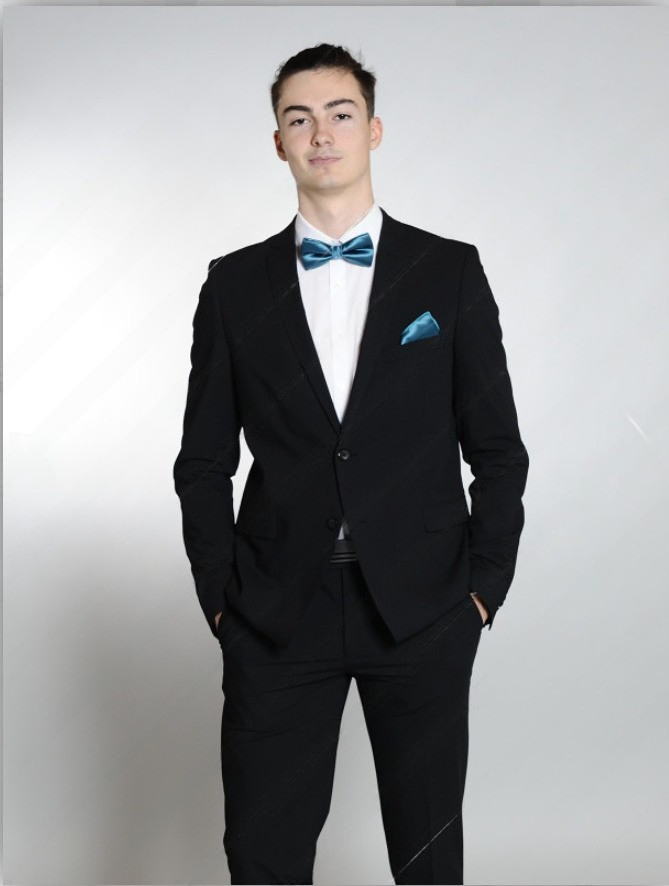
\includegraphics[width=0.28\textwidth]{images/people/leonEdlinger.jpeg} \newline
        Database, Admin-Panel &
        
        \centering
        \textbf{\daAuthorTwo} \newline
        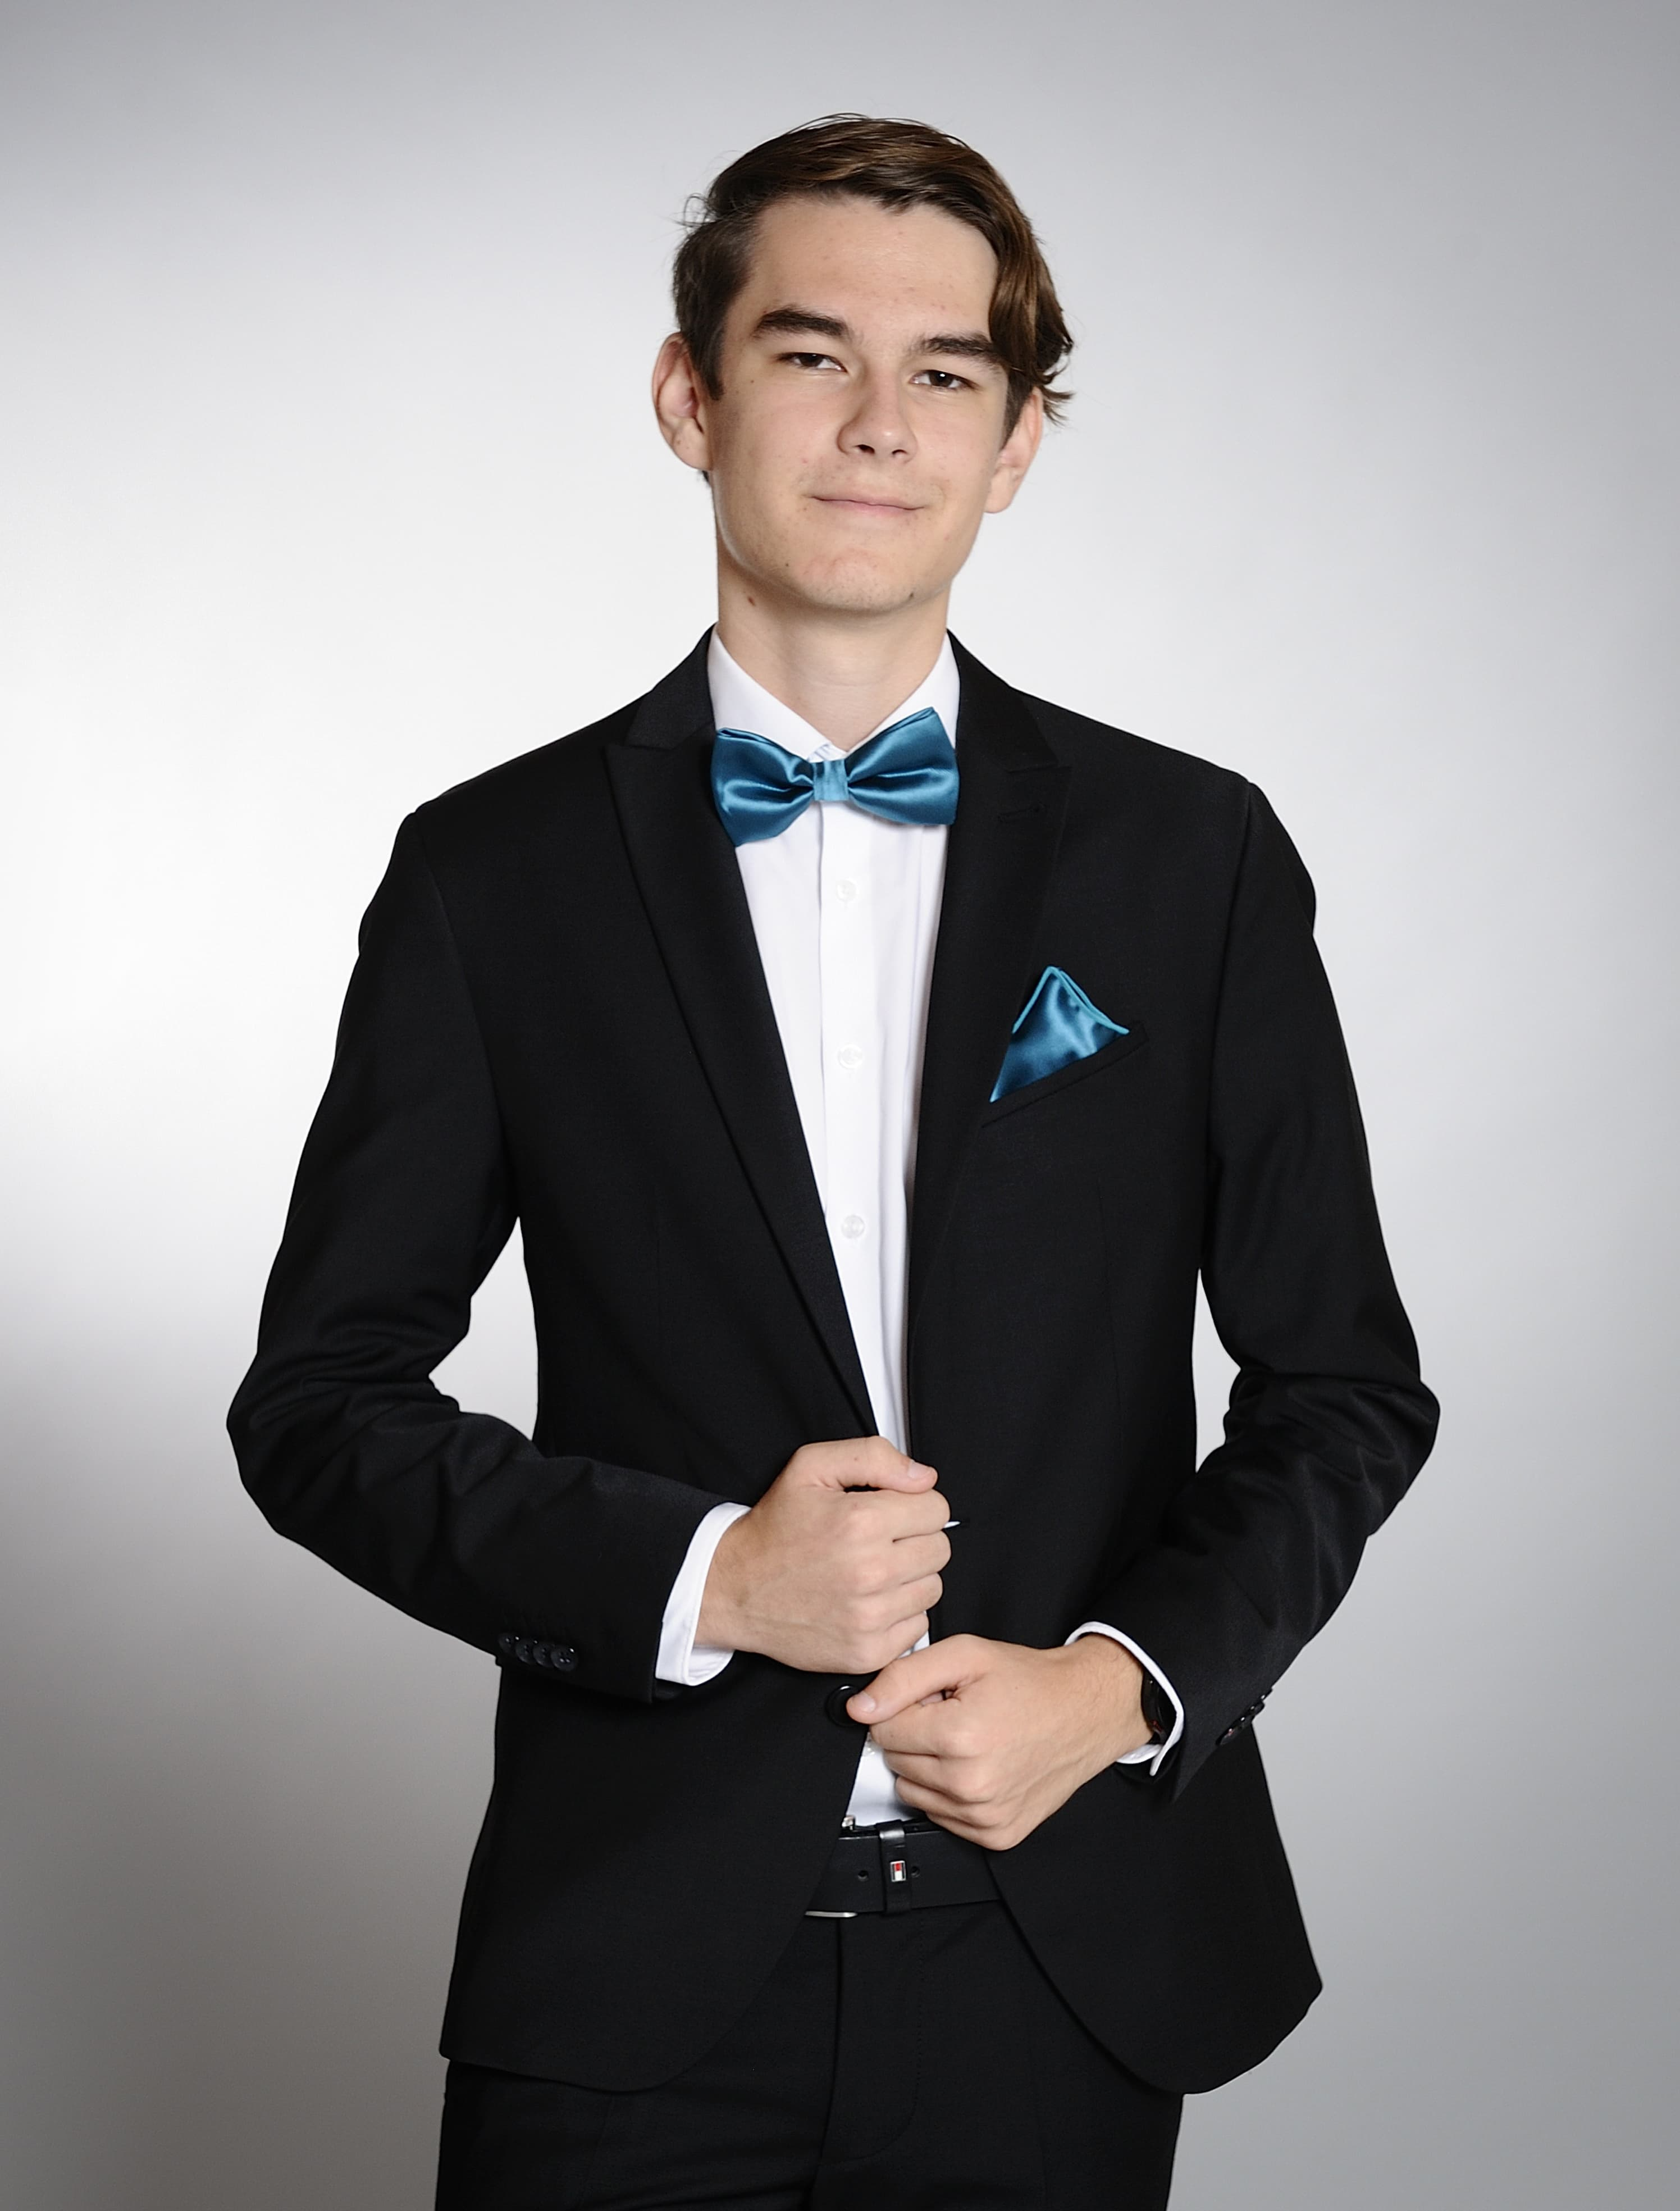
\includegraphics[width=0.28\textwidth]{images/people/paulGigler.jpeg} \newline
        Deployment, Mobile App &
    
        \centering
        \textbf{\daAuthorThree} \newline
        
\includegraphics[width=0.28\textwidth]{images/people/andreasWeissl.jpeg} \newline
        Backend
    \end{tabularx}
    \end{center}

\newpage